% Preamble
% ---
\documentclass{article}

% Packages
% ---
\usepackage{amsmath} % Advanced math typesetting
\usepackage[utf8]{inputenc} % Unicode support (Umlauts etc.)
\usepackage[ngerman]{babel} % Change hyphenation rules
\usepackage{hyperref} % Add a link to your document
\usepackage{graphicx} % Add pictures to your document
\usepackage{listings} % Source code formatting and highlighting
\usepackage{booktabs}

\renewcommand{\figurename}{Figure}
%\usepackage[labelsep=endash]{caption}

\usepackage{xcolor}
\lstset { %
    language=C++,
    backgroundcolor=\color{black!5}, % set backgroundcolor
    basicstyle=\footnotesize,% basic font setting
}



\title{%
	MA226 : Monte-Carlo Simulation\\
	 Generation of Random Numbers from Beta, Normal and Discrete Distributions\\
	 \large Assignment 5}

\date{16-02-2017}

\author{%
	Turkhade Hrushikesh Pramod\\
	150123044	}	

\begin{document}

	\maketitle
	\pagenumbering{gobble}
	
	\newpage
	\pagenumbering{arabic}
	
	\section{Problem 1}
	\paragraph{}
		We have to generate Random Numbers from Normal Distribution using Acceptance Rejection Method. For this, we take $g(x)$ as Double exponential function.
		
		\paragraph{}
		We can find $c$ as follows:
		\paragraph{}
		$f(x)/g(x)=\sqrt{2/\pi}e^{(-x^2/2+\left | x \right |)}<=\sqrt{2e/\pi}=constant$
			
			
		
	\subsection{Source code of the solution}
		\lstinputlisting[language=R,firstline=1,lastline=42]{code/que1.R}
		
		\pagebreak
		\subsubsection{Histograms for the above data}
			\begin{figure}[!ht]
  			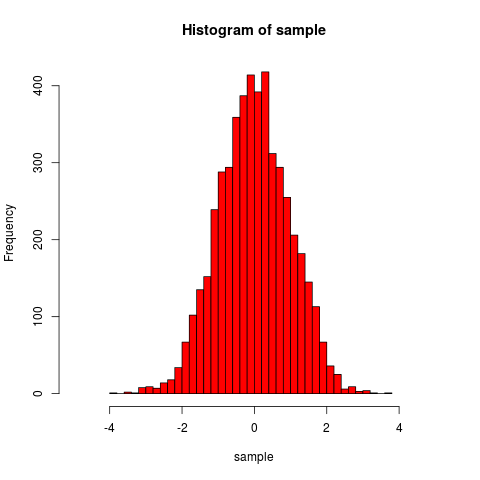
\includegraphics[width=\linewidth]{pic/que1_in_R.png}
 			 \caption{Histogram of Generated Normal Distribution}
  			\label{fig:hist1_1}
		\end{figure}
		
		\subsection{Analysis}
		\paragraph{}
			As we can see from the graph, the histogram is quite similar to standard normal curve. The calculated values of various parameters are as follows:
		
	    \paragraph{}
		\begin{gather}	    
	    Mean=0.016\\
	    Variance=1.056\\
	    Simulated Acceptance Probability=0.755\\
	    Theoritical Acceptance Probability=0.760
	    \end{gather}
	    
	    \pagebreak
	    \section{Problem 2}
	    \paragraph{}
		We have to generate Random Numbers from Half-Standard Normal Distribution using Acception Rejection Method. For this, we take $g(x)$ as Exponential distribution.
		
		\paragraph{}
		We can find $c$ as follows:
		\paragraph{}
		$f(x)/g(x)<=\sqrt{2e/\pi}=constant$
			
		
	\subsection{Source code of the solution}			                       \lstinputlisting[language=R,firstline=1,lastline=36]{code/que2.R}
		
		\pagebreak
		\subsubsection{Histograms for the above data}
			\begin{figure}[!ht]
  			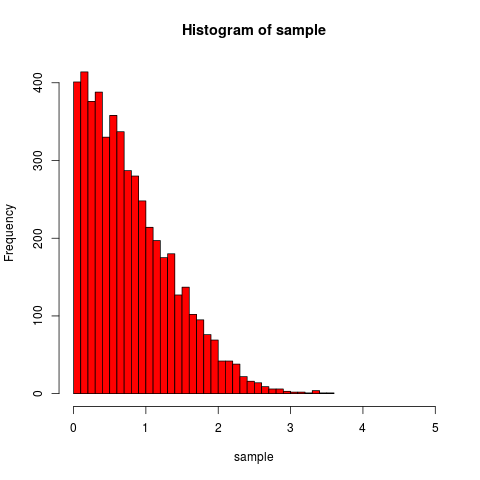
\includegraphics[width=\linewidth]{pic/que2_in_R.png}
 			 \caption{Histogram of Generated Half-Normal Distribution}
  			\label{fig:hist1_1}
		\end{figure}
		
		\subsection{Analysis}
		\paragraph{}
			As we can see from the graph, the histogram is quite similar to half normal curve. The calculated values of various parameters are as follows:
			
	
	    \paragraph{}
		\begin{gather}	    
	    Mean:  0.8041006 \\
Variance:  0.3709299
	    \end{gather}
		
		\pagebreak
		
		
	    \section{Problem 3}
	    \paragraph{}
		We have to generate Random Numbers from Discrete Distribution using Acception Rejection Method and Inverse transform Method. The discrete distribution is as follows
		
		\begin{table}[h!]
      \centering
      \caption{Probabilities of Discrete Distribution}
      \label{tab:table1}
      \begin{tabular}{c c c c c}
        \toprule
        1 &2 &3 &4&5 \\
        \midrule
        0.05& 0.25& 0.45& 0.15& 0.1 \\
        \bottomrule
      \end{tabular}
    \end{table}
		
		
	\subsection{Source code of Inverse-Transform Method}			                       \lstinputlisting[language=R,firstline=1,lastline=25]{code/que3-a.R}
		
	\subsection{Source code of Acceptance Rejection Method}			                       \lstinputlisting[language=R,firstline=1,lastline=25]{code/que3-b.R}	
		
		\subsection{Analysis}
		\paragraph{}
			Following are the values of parameters in Acceptance Rejection Method. But, these are values will be inconsitant as we are generating only 10 numbers. Generatin more numbers will give us more insight on correctness of algorithm
		
	    \paragraph{}
		\begin{gather}
	    Mean:  3.5\\ 
        Variance:  1.166667 
	    \end{gather}
	    
	    \paragraph{}
	    Following are the values of parameters in Inverse-Transform Method. By same reasoning above the values will be inconsitant in multiple runs of the code as number of samples are small.
			
		\paragraph{}
		\begin{gather}
	    Mean:  2.9 \\
        Variance:  0.9888889 
	    \end{gather}
		

\end{document}